\section{Object Detection}

\subsection{Model}

In order to track the kayaker. We must have an real time object detection model. So we choose MobileNet SSD to be our object detection model.
MobileNet separate the convolution process of traditional CNN models into depthwise convolution and pointwise convolution. Then combine the result later to achieve same effect of traditional convolution. But it can drastically reduce the computation.

\begin{figure}[H]
    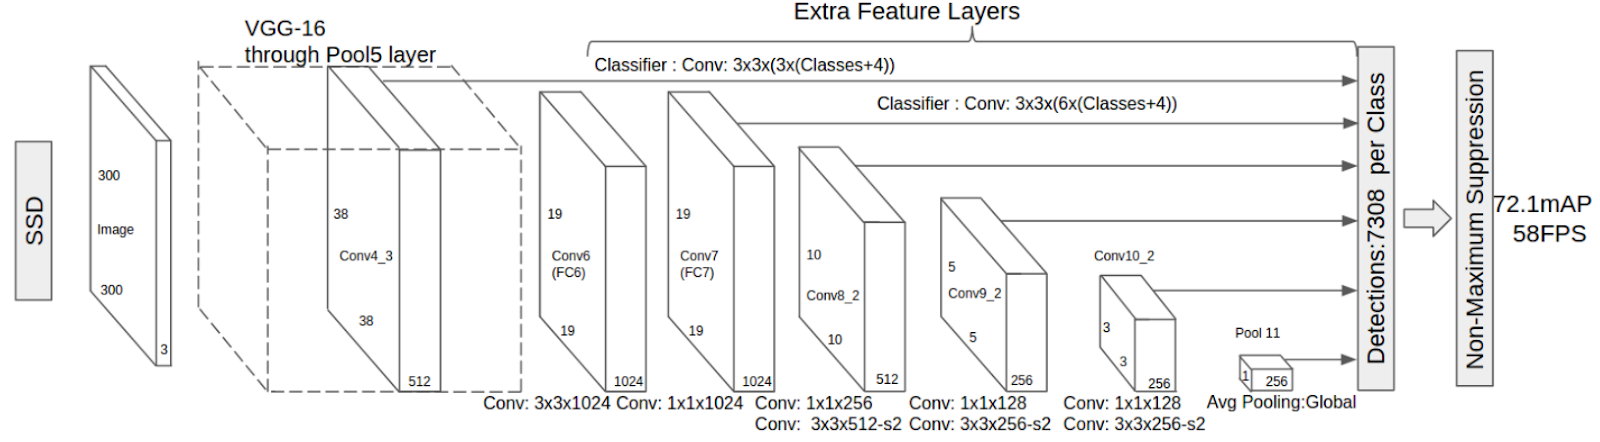
\includegraphics[width=1\columnwidth]{images/mobilenetssd.png}
    \centering
    \caption{SSD model}
    \label{figure:mobilenetssd}
\end{figure}

\subsection{Framework}

We use tensorflow object detection API to train the model. It has plenty of analysis tools for users to monitor training process. Once the model is trained. We use Nvidia jetson-TX2 to run the model. We can get up to 19 frames per second of detection. This is enough to implement kayaker tracking.

\subsection{Data collect and label}

We use 1951 photos of kayaker pictured by onboard picamera on the bamboo lake. Inorder to train a more generalized model. We also try to add 136 photos of kayaker downloaded on google photo. We use labelImg(https://github.com/tzutalin/labelImg) to label the bounding box of the Kayaker.

\begin{figure}[H]
    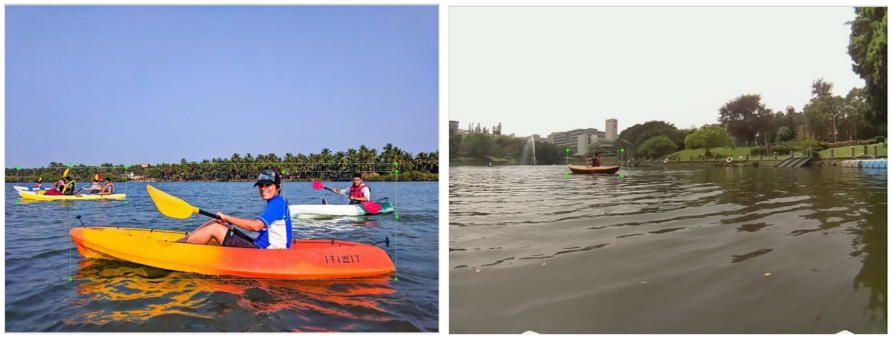
\includegraphics[width=1\columnwidth]{images/kayaker.png}
    \centering
    \caption{kayaker image data}
    \label{figure:kayaker}
\end{figure}

\subsection{Training}

We use GPU:RTX2070 trained for 52 minutes. With learning rate:$4e-3$, batch size:$24$, data split ratiao:$8/2$, epoch:$9265$

\begin{figure}[ht]
    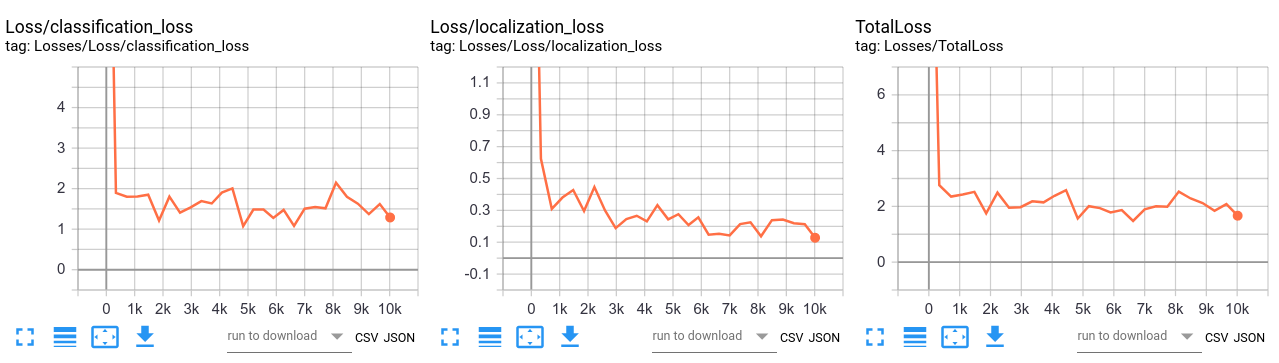
\includegraphics[width=1\columnwidth]{images/train_loss.png}
    \centering
    \caption{training loss}
    \label{figure:training_loss}
\end{figure}

\begin{figure}[H]
    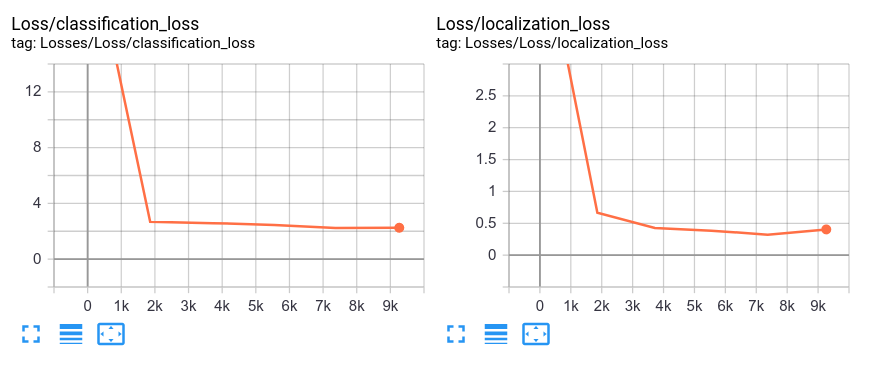
\includegraphics[width=1\columnwidth]{images/eval_loss.png}
    \centering
    \caption{evaluation loss}
    \label{figure:eval_loss}
\end{figure}

\subsection{Model analysis}

We use pr curve at iou=0.5 to analysis the model and compare the difference between pretrained model using COCO dataset boat class and our trained kayaker detection model. AP is improved from $77.09\%$ to $83.40\%$. 

\begin{figure}[H]
    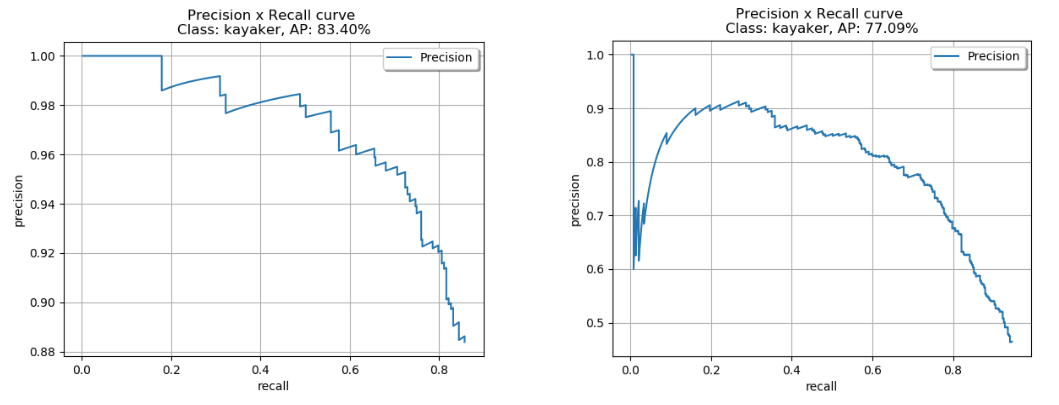
\includegraphics[width=1\columnwidth]{images/kayaker_pr.png}
    \centering
    \caption{left pic is pr curve of kayaker detection model, right pic is pretrained model}
    \label{figure:kayaker_pr}
\end{figure}
\begin{figure}[H]
    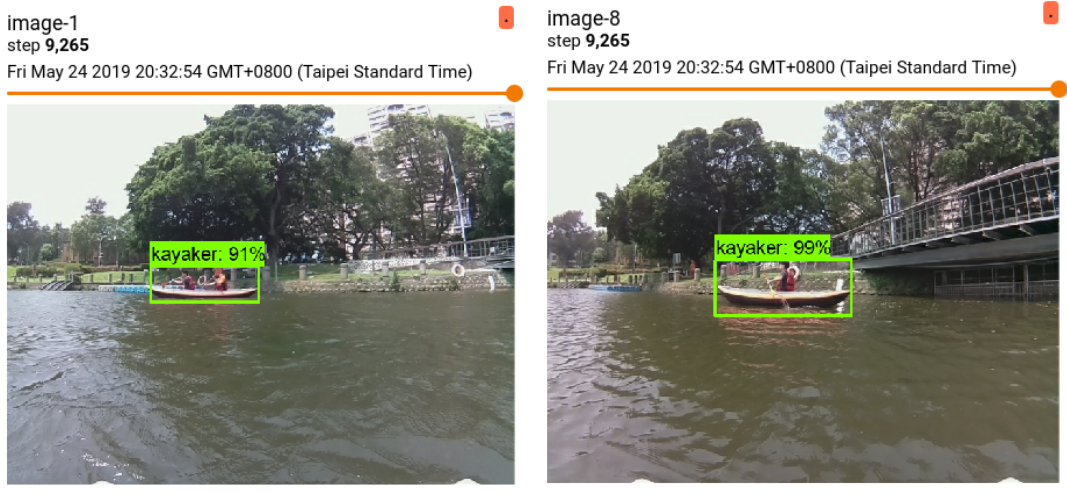
\includegraphics[width=1\columnwidth]{images/kayaker_dt.png}
    \centering
    \caption{detection result}
    \label{figure:kayaker_dt}
\end{figure}

\subsection{Trash detection}

We also try to detect the garbage floating on the water surface. for future applications like garbage collecting.but the challenge is the reflecting light of the water surface and the size of the bottle make it difficult to detect.

\begin{figure}[H]
    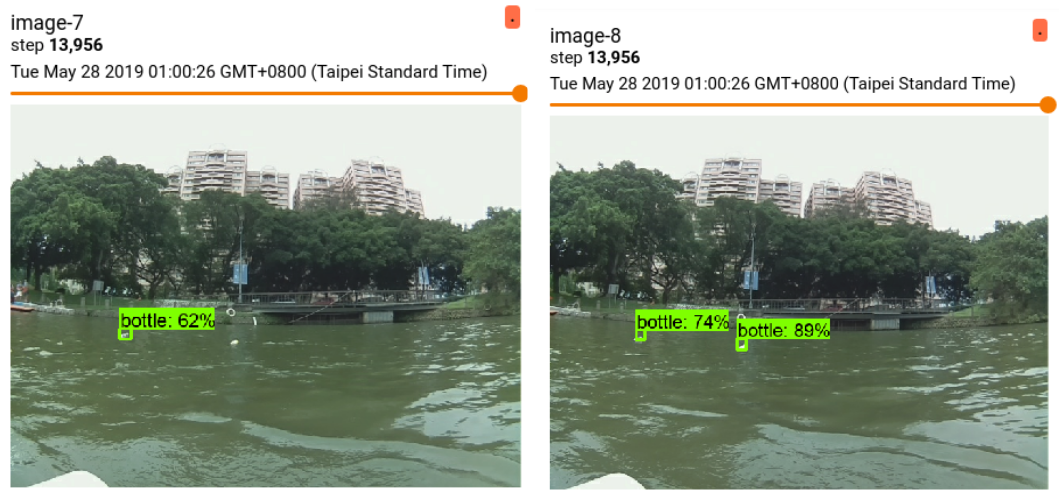
\includegraphics[width=1\columnwidth]{images/bottle.png}
    \centering
    \caption{bottle detection}
    \label{figure:bottle_dt}
\end{figure}


\begin{figure}[H]
    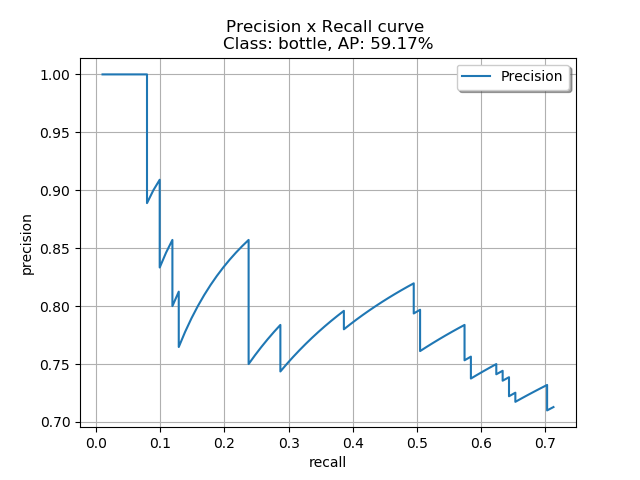
\includegraphics[width=1\columnwidth]{images/bottle_pr.png}
    \centering
    \caption{bottle detection pr curve}
    \label{figure:bottle_pr}
\end{figure}